% Intended LaTeX compiler: pdflatex
\documentclass[10pt,a4paper,UTF8]{article}
\usepackage{zclorg}
\author{张朝龙}
\date{}
\title{练习:本证向量与上三角阵}
\hypersetup{
 pdfauthor={张朝龙},
 pdftitle={练习:本证向量与上三角阵},
 pdfkeywords={},
 pdfsubject={},
 pdfcreator={Emacs 25.0.50.1 (Org mode 9.0.5)},
 pdflang={English}}
\begin{document}

\maketitle
\tableofcontents
\titlepic{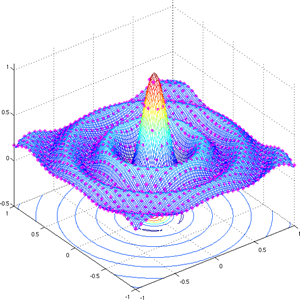
\includegraphics[scale=0.25]{../../img/sinc.PNG}}

\section{5.B.1}
\label{sec:orgd09a881}


\begin{problem}
设\(T\in \mathcal{L}(V)\)且存在正整数\(n\)使得\(T^{n} = 0\):
\begin{enumerate}
\item 证明\(I-T\)是可逆的,且其逆为\((I-T)^{-1} = I + T + \ldots + T^{n-1}\)
\item 解释一下如何想到上面公式。
\end{enumerate}
\end{problem}

\begin{answer}
\begin{eqnarray}
\label{eq:1}
(I-T)(I + T + \ldots T^{n-1})&=&(I + T + \ldots T^{n-1}) - (T +T^{2} + \ldots +T^{n-1} + T^{n} )  \\
&=& I
\end{eqnarray}
\end{answer}
\section{5.B.2}
\label{sec:orgdd6d2e6}


\begin{problem}
设\(T\in \mathcal{L}(V)\)且\((T-2I)(T-3I)(T-4I) = 0\),设\(\lambda\)是\(T\)的本征值,证明\(\lambda= 2\) 或者 \(\lambda = 3\),或者\(\lambda = 4\)
\end{problem}

\begin{answer}
见定理5.21的证明过程。
\end{answer}
\section{5.B.3}
\label{sec:org4dbdb28}


\begin{problem}
设\(T\in \mathcal{L}(V)\),\(T^{2} = I\),且\(-1\)不是\(T\)的本征值。证明\(T=I\)
\end{problem}

\begin{answer}
由\(T^{2} = I\)得\((T-I)(T+I) = 0\),则\(T\)有特征值\(1\)或者\(-1\),又因为\(-1\)不是\(T\)的特征值,则\(1\)是\(T\)的唯一特征值,所以\(T = I\)
\end{answer}

\section{5.B.4}
\label{sec:org2161f05}


\begin{problem}
设\(P\in \mathcal{L}(V)\),\(P^{2} = P\),证明\(V = \mathrm{null} P \oplus \mathrm{range} P\)
\end{problem}

\begin{answer}
因为\(P^{2} = P\),则\(P= 0\)或者\(P=I\)。

当\(P=0\)时,\(\mathrm{range}P = \{0\}\),\(\mathrm{null}P = V\),因此\(V = \mathrm{null} P \oplus \mathrm{range}P\);
当\(P=I\)时,\(\mathrm{null}P = \{0}\),\(\mathrm{range}P = V\),同样结论成立。

综上命题得证。
\end{answer}

\section{5.B.5}
\label{sec:orgaa9300c}


\begin{problem}
设\(S.T\in \mathcal{L}(V)\)且\(S\)是可逆的。设\(p\in \mathcal{P}(\mathbf{F})\)是多项式。证明\(p(STS^{-1}) = Sp(T)S^{-1}\)
\end{problem}

\begin{answer}
根据多项式定义:
\begin{equation}
\label{eq:3}
p(x) = a_{0} + a_{1}x + a_{2}x^{2} + \ldots
\end{equation}
则有\(p(STS^{-1})\) 为:
\begin{equation}
\label{eq:4}
p(STS^{-1}) = a_{0}I + a_{1}STS^{-1} + a_{2}(STS^{-1}STS) + \ldots
\end{equation}
上式经过整理可以变为:
\begin{eqnarray}
\label{eq:5}
p(STS^{-1}) &=& a_{0}I + a_{1}STS^{-1} + a_{2}(STS^{-1}STS) + \ldots \\
&=& a_{0}SIS^{-1} + a_{1}STS^{-1} + a_{2}ST^{2}S^{-1} + \ldots \\
&=& S(a_{0}I + a_{1}T + a_{2}T^{2} + \ldots )S^{-1} \\
&=&Sp(T)S^{-1}
\end{eqnarray}
\end{answer}

\section{5.B.6}
\label{sec:org1243dcd}


\begin{problem}
设\(T\in \mathcal{L}(V)\)且\(U\)是\(V\)的在\(T\)下不变的子空间,证明对每个多项式\(p\in \mathcal{P}(\mathbf{F})\)都有\(U\)在\(p(T)\)下不变。
\end{problem}

\begin{answer}
根据多项式定义,对多项式的每一项进行分析即可。
\end{answer}

\section{5.B.7}
\label{sec:org71ffdbd}


\begin{problem}
设\(T\in \mathcal{L}(V)\),证明\(9\)是\(T^{2}\)的本征值当且仅当\(3\)或者\(-3\)是\(T\)的本征值。
\end{problem}

\begin{answer}
假设\(\lambda\)是\(T\)的一个特征值,且对应的特征值向量是\(v\),则\[Tv = \lambda v\],所以:\[T^{2}v = T(\lambda v) = \lambda^{2}v\] 对此进行扩展有:\[p(T)v = p(\lambda)v\]
因此如果\(9\)是\(T^{2}\)的特征值则有:\[T^{2}v = 9v \]进而有:\[(T-3I)(T+3I)v = 0\]所以\(T-3I\)或者\(T+3I\)至少有一个不是单射,所以\(3\)或者\(-3\)是\(T\)的特征值。
\end{answer}

\section{5.B.8}
\label{sec:org8d7e15e}


\begin{problem}
找出一个\(T\in \mathcal{L}( \mathbf{R}^{2})\)使得\(T^{4} = -I\)
\end{problem}

\begin{answer}
\begin{equation}
\label{eq:6}
T(x,y) = (\frac{\sqrt{2}}{2} x - \frac{\sqrt{2}}{2} y, \frac{\sqrt{2}}{2}x + \frac{\sqrt{2}}{2} y)
\end{equation}
\end{answer}
\section{5.B.9}
\label{sec:org07719f5}


\begin{problem}
设\(V\)是有限维的,\(T\in \mathcal{L}(V)\),\(v\in V,v\neq 0\)。设\(p\)是使得\(p(T)v = 0\)的次数最小的非零多项式。证明\(p\)的每个零点都是\(T\)的本征值。
\end{problem}
\section{5.B.10}
\label{sec:org7742542}


\begin{problem}
设\(T\in \mathcal{L}(V)\),\(v\)是\(T\)的相应于本征值\(\lambda\)的本证向量。设\(p\in \mathcal{P}(\mathbf{F})\),证明\(p(T)v = p(\lambda)v\)
\end{problem}

\begin{answer}
我们证明过\(T^{n}v = \lambda^{n}v\),因此对于:\[p = \sum_{n=1}^{k}a_{n}x^{n}\]有:
\begin{equation}
\label{eq:7}
p(T)v = (\sum_{n=0}^{k}a_{n}T^{n})v = \sum_{n=0}^{k}a_{n}\lambda^{n}v = p(\lambda)v
\end{equation}
\end{answer}
\section{5.B.11}
\label{sec:org3701732}


\begin{problem}
设\(\mathbf{F}= \mathbf{C}\),\(T\in \mathcal{L}(V)\),\(p\in \mathcal{P}(\mathbf{C})\)是多项式,\(\alpha \in \mathbf{C}\),证明\(\alpha\)是\(p(T)\)的本征值当且仅当\(T\)有一个本征值\(\lambda\)使得\(\alpha = p(\lambda)\)
\end{problem}

\begin{answer}
首先假设\(\alpha\)是\(p(T)\)的本征值,那么\(p(T) - \alpha I\)不是单射,把多项式\(p(z) - \alpha\)因式分解:
\begin{equation}
\label{eq:8}
p(z) - \alpha  = c(z-\alpha_{1})\ldots (z-\lambda_{m})
\end{equation}
上式意味着:
\begin{equation}
\label{eq:9}
p(T) - \alpha I = c(T-\lambda_{1} I) \ldots (T-\lambda_{m} I)
\end{equation}
因为\(p(T)  - \alpha I\)不是单射,所以对于某个\(j\),\(T - \lambda_{j} I\)不是单射。换句话说\(\lambda_{j}\)是\(T\)的特征值。所以\(p(z) - \alpha  = 0\),即\(\alpha = p(z)\)

另一方面,假设存在某个特征值\(\lambda\)使得\(\alpha = p(\lambda)\),所以存在非零向量\(v\in V\),满足:
\begin{equation}
\label{eq:10}
Tv= \lambda v
\end{equation}
重复对左侧进行\(T\)映射,所以:
\begin{equation}
\label{eq:11}
p(T)v = p(\lambda)v = av
\end{equation}
即\(\alpha\)是\(p(T)\)的一个特征值。
\end{answer}
\section{5.B.12}
\label{sec:org75dccdf}


\begin{problem}
证明若将\(\mathbf{C}\)换成\(\mathbf{R}\),上题的结论将不在成立。
\end{problem}

\begin{answer}
定义\(T\in \mathcal{L}(\mathbf{R}^{2})\)为 \(T(x,y) = (-y,x)\),定义\(p\in \mathcal{P}(\mathbf{R})\)为\(p(x) = x^{2}\),那么\(p(T) = T^{2} = -I\)因此\(-1\)是\(p(T)\)的特征值,但是\(T\)没有实数域上的特征值。
\end{answer}

\section{5.B.13}
\label{sec:org2574b53}


\begin{problem}
设\(W\)是复向量空间,并设\(T\in \mathcal{L}(W)\)没有本征值,证明:\(W\)在\(T\)下不变的子空间是\(\{0\}\)或者是无限维的。
\end{problem}

\begin{answer}
反证法
\end{answer}
\section{5.B.14}
\label{sec:org1ef4380}


\begin{problem}
给出一个算子,它关于某个基的矩阵的对角线上只有\(0\),但这个算子是可逆的。
\end{problem}

\begin{answer}
这个很容易,对于二维空间有基\(e_{1},e_{2}\) ,定义算子\(T\in \mathcal{L}(\mathbf{R}^{2})\):
\begin{eqnarray}
\label{eq:12}
Te_{1}&=&e_{2} \\
Te_{2}&=&e_{1}
\end{eqnarray}
显然这个映射对应的矩阵对角线上全是\(0\),但是它是可逆的。
\end{answer}
\section{5.B.15}
\label{sec:org46cfd36}


\begin{problem}
给出一个算子,它关于某个基的矩阵的对角线上全是非零值,但是这个算子是不可逆的。
\end{problem}

\begin{answer}
定义矩阵:
\begin{equation}
\label{eq:13}
\begin{bmatrix}
1 & 1 \\
1 & 1
\end{bmatrix}
\end{equation}
显然\(T(0,1) = T(1,0) = (1,1)\)
\end{answer}
\section{5.B.16}
\label{sec:orgba79912}


\begin{problem}
利用将\(p\in \mathcal{P}_{n}(\mathbf{C})\)变为\((p(T)) v\in V\)的线性映射,证明:复向量空间上的算子都有本征值。
\end{problem}

\begin{answer}
定义\(\varphi(p) = p(T)v\):
\begin{equation}
\label{eq:14}
\varphi: \mathcal{P}_{n}(\mathbf{C}) \rightarrow V
\end{equation}
那么\(\varphi\)是一个线性映射,注意:\(\dim \mathcal{P}_{n}(\mathbf{C}) = n+1\)且\(\dim V = n\)所以\(\varphi\)不是单射,所以存在非零元素\(p\)使得\(p(T)v = 0\).

剩下的和5.21的证明过程一样。
\end{answer}
\end{document}
